% HUMAN_REPRODUCTION_V4_2026_10_29
\documentclass[11pt,a4paper]{article}
\usepackage[margin=25mm]{geometry}
\usepackage[T1]{fontenc}
\usepackage{mathpazo,amsmath,amssymb,graphicx,booktabs,longtable,array,caption,setspace,microtype}
\usepackage[authoryear,round]{natbib}
\usepackage[hidelinks]{hyperref}
\usepackage{fancyhdr}
\usepackage{placeins}
\usepackage[mathlines]{lineno}
\doublespacing
\setlength{\parskip}{4pt}
\setlength{\parindent}{0pt}
\captionsetup{font=small,labelfont=bf}
\pagestyle{fancy}\fancyhf{}\fancyhead[L]{\small PCOS infertility and reference composition}\fancyhead[R]{\thepage}
\setlength{\headheight}{14pt}
\setlength{\emergencystretch}{2em}
\newcommand{\ASPR}{\mathrm{ASPR}}
\title{Reference-country composition and age-standardized PCOS-attributed infertility contrasts: China and 18 G20 countries, 1990--2023}
\author{XX Author$^{1}$, XX Author$^{2}$, XX Corresponding Author$^{1,*}$\\
{\small $^{1}$XX Department, XX Institution, XX City, XX Country, XX Postal code}\\
{\small $^{2}$XX Department, XX Institution, XX City, XX Country, XX Postal code}\\
{\small $^{*}$Correspondence: XX email; ORCID: XX}}
\date{29 October 2026}

\begin{document}
\maketitle\thispagestyle{fancy}
\linenumbers
\begingroup\sloppy
\begin{abstract}
\noindent\textbf{STUDY QUESTION:} How much of the 1990--2023 change in the China-minus-reference age-standardized prevalence difference for total PCOS-attributed infertility is allocated to changing within-age country shares in a contemporaneously population-pooled 18-country reference?

\noindent\textbf{SUMMARY ANSWER:} Changing reference-country shares contributed +88.65 per 100,000 to the +151.54 change in the modeled difference, equivalent to 58.5\% of the signed net change.

\noindent\textbf{WHAT IS KNOWN ALREADY:} GBD studies describe PCOS-attributed infertility burden across countries and time. Fixing age-standardization weights does not also fix country population shares within each age group of a multinational reference.

\noindent\textbf{STUDY DESIGN, SIZE, DURATION:} This exploratory ecological secondary analysis used GBD 2023 estimates for China and 18 other sovereign G20 countries, seven five-year female age groups spanning 15--49 years, and 34 years, 1990--2023. No individual participants were recruited.

\noindent\textbf{PARTICIPANTS/MATERIALS, SETTING, METHODS:} Matched GBD prevalence counts and female populations yielded age-specific rates per 100,000 females. Fixed age weights were normalized over ages 15--49. The primary estimand was the change in the China-minus-contemporaneous-reference difference for total PCOS-attributed infertility. An established symmetric identity separated Chinese rate, reference-country rate and reference-share components. UN WPP 2024 replaced reference shares only. Subtypes, fixed-1990 shares, equal-country weights and deterministic sensitivity scenarios addressed secondary questions.

\noindent\textbf{MAIN RESULTS AND THE ROLE OF CHANCE:} China's total rate increased from 333.56 to 605.08 and the reference rate from 606.48 to 726.45 per 100,000. The difference moved from $-272.92$ to $-121.38$: Chinese rates, reference rates and shares contributed $+271.51-208.62+88.65=+151.54$ (rounded). UN shares gave +86.76 for the share component (57.6\% of +150.69). For secondary infertility in 2023, the difference was +2.16 under contemporaneous GBD shares, $-47.99$ under fixed-1990 shares and $-127.89$ under equal-country weights. Jointly aligned GBD posterior draws were unavailable; no derived uncertainty intervals or significance tests are reported.

\noindent\textbf{LIMITATIONS, REASONS FOR CAUTION:} These empirical quantities are conditional on GBD model point estimates and rounded published age weights. The uncertainty of component magnitudes and near-zero contrast signs remains unquantified. Scenario ranges are not uncertainty intervals. The 58.5\% ratio uses a signed net denominator with cancellation, rather than a fraction of women or disease. The G20 reference is economically selected and does not represent a clinical control group or the world.

\noindent\textbf{WIDER IMPLICATIONS OF THE FINDINGS:} Researchers monitoring national reproductive-health estimates against pooled international populations should state the comparator weights and report absolute rate and composition components. The mathematical persistence of within-age country composition after age standardization is distinct from its estimated magnitude in these data. Benchmark-dependent contrasts do not establish improved care, causal effects or individual infertility risk.

\noindent\textbf{FUNDING:} XX: verified funding sources and funder roles to be completed by the authors at submission.

\noindent\textbf{DISCLOSURES:} XX: author-specific disclosures to be completed at submission.

\noindent\textbf{TRIAL REGISTRATION NUMBER:} Not applicable; this is a secondary analysis of aggregate estimates, not a clinical trial.
\end{abstract}
\endgroup

\textbf{Keywords:} Polycystic Ovary Syndrome; Infertility, Female; Prevalence; Age Distribution; Population Dynamics.

\section{Introduction}
Polycystic ovary syndrome (PCOS) is relevant to reproductive health and individualized care \citep{pcos}. Infertility attributed to PCOS in the Global Burden of Disease (GBD) study is a modeled cause-specific impairment outcome, distinct from general PCOS prevalence and infertility risk among couples trying to conceive \citep{gbd}. A practical use of these estimates is to monitor a country's trajectory against a multinational population. Such monitoring requires a definition of whose experience the reference represents at each date.

Liu and colleagues described GBD 2019 PCOS-attributed infertility prevalence, disability and trends at global, regional and national levels \citep{liu_pcos2024}. Liang and colleagues used GBD 2021 and decomposed burden changes into population growth, ageing and epidemiological components \citep{liang_burden2025}. Another analysis examined China and worldwide trends using GBD 2021 \citep{liang_trend2026}. These objectives differ from accounting for a national standardized-rate contrast against an explicitly constructed 18-country pool (Supplementary Table~S9). A count decomposition includes population size and age structure, whereas our contrast decomposition holds the age standard fixed and isolates changing country shares within each age. We do not infer that these earlier studies used our pooling rule or made an erroneous comparison.

A contemporary population-pooled reference is useful when the question concerns the population mix actually represented at each date. Yet the same fixed list of countries can represent a different within-age country mix over time. For example, an increased share for a country with a lower age-specific rate can lower the pooled reference even if each country's rate is unchanged. Fixed age-standardization weights do not remove this second level of composition. A narrowing national gap can therefore coexist with increasing national and reference rates; it cannot by itself establish improved reproductive health.

Our primary objective was to quantify the 1990--2023 change in China's total PCOS-attributed infertility standardized prevalence difference against a contemporaneously population-pooled reference of 18 other sovereign G20 countries, and its symmetric allocation to Chinese rates, reference-country rates and within-age reference-country shares. We apply established Kitagawa-type accounting rather than propose a new method \citep{kitagawa}. Secondary objectives assess demographic-source sensitivity, infertility subtypes and alternative benchmark questions. The fixed G20 country set is interpretable for monitoring but is neither globally representative, a matched clinical control nor a normative treatment target.

\section{Materials and methods}
\subsection{Design, data and outcome}
This ecological secondary analysis used GBD 2023 Results Tool exports obtained on 25 October 2026 \citep{results}. We included females aged 15--49, seven five-year ages and 1990--2023. The reference countries were Argentina, Australia, Brazil, Canada, France, Germany, India, Indonesia, Italy, Japan, Republic of Korea, Mexico, Russian Federation, Saudi Arabia, South Africa, T\"urkiye, United Kingdom and United States of America. China was always excluded from the reference; regional organizations were excluded.

We selected prevalence (measure 5), PCOS (cause 605), total infertility (impairment 198), primary infertility (220) and secondary infertility (221), with endometriosis (607) as a comparator cause. Rates used all females in each age group as the denominator. GBD's survey-based infertility framework includes desire for a child, union duration, contraceptive use and previous live birth, with heterogeneous sources harmonized within its model \citep{gbd}. These estimates must not be read as a uniformly measured 12-month clinical infertility rate or individual reproductive risk.

Matched female populations came from the same GBD release. We calculated age-specific prevalence per 100,000 as $r_{catk}=10^5 C_{catk}/P_{cat}$ for country $c$, age $a$, year $t$ and infertility type $k$. We required complete, unique country--age--year cells, nonnegative finite values, primary-plus-secondary additivity and agreement with separately downloaded official endpoint Rate values. Source files and hashes are specified in the reproducibility archive.

\subsection{Primary estimand and age-standardized reference}
The primary estimand is $\Delta D_{\mathrm{total}}=D_{2023,\mathrm{total}}-D_{1990,\mathrm{total}}$ under contemporaneous GBD reference-country population shares. The population is females aged 15--49 in China and the fixed 18-country reference; the outcome is modeled total PCOS-attributed infertility prevalence, with all females as denominator. The contrast is a difference per 100,000 after restricted-age standardization. Its symmetric components are descriptive allocations of that same change. Subtype contrasts and the UN, fixed-1990 and equal-country specifications are secondary; they do not redefine the primary target.

Published GBD 2023 age weights reproduced to six decimals were normalized to sum to one over ages 15--49 \citep{chen}. They remained fixed throughout. The original machine-precision IHME standard file was unavailable. These are restricted-age standardized rates, not all-age standardized rates.
\begin{align}
 s_{cat}&=\frac{P_{cat}}{\sum_{j\in R}P_{jat}}, &
 A_{Rtk}&=\sum_a w_a\sum_{c\in R}s_{cat}r_{catk},\\
 A_{Ctk}&=\sum_a w_ar_{Catk}, &D_{tk}&=A_{Ctk}-A_{Rtk}.
\end{align}
Here $R$ is the fixed set of 18 reference countries, and $w_a$ is the normalized standard age weight. Country shares $s_{cat}$ vary within age and year even though $w_a$ does not. Thus fixing the country list and the age standard does not fix reference composition. This follows from the pooling equation independently of any GBD estimate; whether the resulting effect is large in these data is an empirical question. Reference rates were pooled within age before standardization.

\subsection{Symmetric descriptive accounting}
For start year 0 and end year $T$, we applied the symmetric product decomposition \citep{kitagawa}:
\begin{align}
 \Delta D_k &=X_k+Q_k+S_k,\\
 X_k&=\sum_a w_a(r_{CaTk}-r_{Ca0k}),\\
 Q_k&=-\sum_a w_a\sum_{c\in R}\frac{s_{ca0}+s_{caT}}{2}(r_{caTk}-r_{ca0k}),\\
 S_k&=-\sum_a w_a\sum_{c\in R}\frac{r_{ca0k}+r_{caTk}}{2}(s_{caT}-s_{ca0}).
\end{align}
$X$ measures changes in Chinese modeled rates, $Q$ changes in reference-country modeled rates, and $S$ changes in reference-country population shares. Averaging the two replacement orders allocates the product interaction symmetrically. The identity is exact before rounding and additive across ages and infertility types. Algebraically, $S=0$ if all within-age country shares are unchanged. It is also zero if the mean of each country's two endpoint rates is identical across countries within each age, because share changes sum to zero. These are properties of the identity, not empirical discoveries, statistical null tests or guarantees of a nonzero component in other settings.

We emphasize absolute components. The descriptive ratio $100S/\Delta D$ uses a signed net change in its denominator. Opposing components can cancel, so this ratio can be unstable, exceed 100\% or reverse sign. It is not a fraction of women or cases, an explained proportion of disease, an attributable fraction or a causal effect. If $\Delta D$ is near zero, absolute components are preferable. Subtype contributions and country-share contributions overlap and must not be added as separate explanations.

\subsection{Population source and benchmark questions}
The official UN WPP 2024 historical mid-year population table supplied females in the same 4,522 country--age--year cells \citep{wpp2024}. Values in thousands were converted to persons. We substituted only UN reference-country shares within age and year; GBD disease rates and standard age weights remained unchanged. We did not divide GBD cases by UN populations. WPP projections from 2024 onward were excluded. The demographic-source comparison is not an independent disease-rate validation, and underlying population evidence may overlap.

We compared three benchmark definitions, summarized below. The contemporary GBD pool is primary because it matches our monitoring question. The other definitions deliberately change the reference population and therefore the estimand; none is intrinsically the correct target for all questions. A fixed-share sensitivity follows one replacement path and is not the symmetric $S$ component.

\begin{quote}\small\setstretch{1.15}
\textbf{Reading the three benchmarks.} Current-year shares compare China with the contemporaneous population-pooled reference. Fixed-1990 shares compare China with current reference-country rates reweighted to the countries' 1990 within-age mix. Equal-country weights compare China with the within-age arithmetic mean across 18 countries. These are alternative descriptive estimands, not three estimates of a single clinical or causal quantity.
\end{quote}

\subsection{Sensitivity, uncertainty and reproducibility}
We repeated the decomposition under both population sources, omitting each reference country, restricting ages to 20--49 with renormalized age weights, starting in 1990 or 2010, and ending in 2021, 2022 or 2023. We also summed adjacent-year decompositions over 1990--2023. All $2^7=128$ corner perturbations of published unnormalized age weights by $\pm0.5\times10^{-6}$ assessed rounding sensitivity. Country exclusions, alternative weights, accounting paths and rounding envelopes are deterministic scenario checks, not confidence intervals. Detailed endometriosis terminal-year checks, a secondary cause contrast related to broader attribution studies \citep{xu}, are confined to Supplementary data.

The existing exports contain marginal summaries and no posterior draw columns. Confirmed jointly aligned draws across countries, ages, years and infertility types were not available in the accessible inputs. We therefore report derived point estimates without propagated uncertainty intervals or significance tests. Marginal lower and upper bounds cannot recover their dependence; we did not sum them, assume independent draws or bootstrap G20 countries as a substitute. If aligned draws become available, the complete pooling and decomposition must be repeated within each verified draw before summarizing posterior quantiles.

These exploratory analyses were not externally preregistered. Core estimates were independently recomputed in Python 3.12 and base R 4.6 and compared numerically. Code, aggregate results, input specifications and a reproducibility entry point are available in the versioned archive \citep{repository}. Computational checks establish implementation consistency, not independent disease-model validity. The supplement maps applicable GATHER items and identifies incomplete uncertainty reporting \citep{gather}.

\subsection{Ethical approval}
Public aggregate GBD estimates and UN demographic data were analysed without individual participant records. XX: institutional ethics-review applicability or exemption determination to be confirmed by the responsible author. No ethics approval number is asserted.

\subsection{Use of artificial intelligence}
OpenAI-assisted tools supported coding, drafting and technical checks. No artificial observations or posterior draws were substituted for the downloaded study data. Human review of scientific interpretation, code and author declarations remains necessary; the tool is not an author.

\section{Results}
\subsection{Coverage and PCOS contrasts}
The GBD population and UN subset each covered 4,522 cells; the prevalence analysis contained 27,132 country--age--year--cause--type cells. Primary plus secondary modeled counts reproduced total counts to within $5.83\times10^{-10}$ cases. Across 1,064 independently exported subtype endpoint rates, reconstruction error was at most $1.16\times10^{-11}$ per 100,000. R and Python core outputs differed by at most $5.69\times10^{-13}$ across the four comparison tables. These are computational consistency checks rather than validation of the underlying disease model.

China's PCOS-attributed total infertility standardized rate increased from 333.56 to 605.08 per 100,000, while the population-pooled reference increased from 606.48 to 726.45 (Table~\ref{tab:pcos}; Figure~\ref{fig:trends}). The difference changed from $-272.92$ to $-121.38$ and the ratio from 0.550 to 0.833. Both rates increased, so a narrowing negative contrast does not establish improved reproductive health.

\begin{table}[htbp]\centering\small\setstretch{1.15}
\caption{PCOS-attributed infertility rates and contrasts under contemporary GBD population shares.}\label{tab:pcos}
\begin{tabular}{llrrrr}\toprule
Type & Year & China & Reference & Difference & Ratio\\\midrule
Total & 1990 & 333.56 & 606.48 & -272.92 & 0.550\\
Total & 2023 & 605.08 & 726.45 & -121.38 & 0.833\\
Primary & 1990 & 44.70 & 214.64 & -169.94 & 0.208\\
Primary & 2023 & 97.35 & 220.89 & -123.54 & 0.441\\
Secondary & 1990 & 288.86 & 391.84 & -102.98 & 0.737\\
Secondary & 2023 & 507.72 & 505.56 & +2.16 & 1.004\\
\bottomrule
\end{tabular}
\caption*{Rates and differences are per 100,000 females, standardized within ages 15--49. Difference is China minus reference. All are model point estimates without propagated posterior intervals.}
\end{table}

\subsection{Absolute decomposition before percentages}
The 1990--2023 change in the total contrast was
\begin{equation}
 \underbrace{+271.51}_{X}\;\underbrace{-208.62}_{Q}\;\underbrace{+88.65}_{S}
 =\underbrace{+151.54}_{\Delta D}\quad\text{per 100,000},
\end{equation}
with displayed rounding (Table~\ref{tab:decomp}; Figure~\ref{fig:decomp}). Chinese rate changes and reference-share changes moved the signed difference upward, while reference-country rate changes offset them. The country-share term was 58.5\% of the signed net change; this denominator is smaller because positive and negative terms cancel.

The country-share component was +88.11 ending in 2021 and +86.74 ending in 2022. The annual-chained component was +87.11 (57.5\%). Across 18 country exclusions and restriction to ages 20--49, the GBD 1990--2023 country-share ratio ranged from 39.8\% to 67.9\% (Supplementary data, Table~S2 and Figure~S3). A substantial contribution persisted, but it was not a majority in every specification. These limits describe specified benchmark sensitivities and are not an uncertainty interval.

Secondary infertility contributed +105.14 and primary infertility +46.40 to the +151.54 total change. The secondary contribution was 69.4\% of the signed net change. Its country-share component was +56.81, compared with +31.84 for primary infertility. The 69.4\% subtype ratio and 58.5\% country-share ratio describe intersecting partitions of the same change and must not be added.

\begin{table}[htbp]\centering\small\setstretch{1.15}
\caption{Symmetric PCOS contrast-change decomposition, 1990--2023, by population source.}\label{tab:decomp}
\setlength{\tabcolsep}{4pt}
\begin{tabular}{llrrrr}\toprule
Type & Shares & China rates $X$ & Ref. rates $Q$ & Ref. shares $S$ & Net $\Delta D$\\\midrule
Total & GBD & +271.51 & -208.62 & +88.65 & +151.54\\
Total & UN WPP & +271.51 & -207.59 & +86.76 & +150.69\\
Primary & GBD & +52.65 & -38.09 & +31.84 & +46.40\\
Primary & UN WPP & +52.65 & -37.75 & +30.13 & +45.02\\
Secondary & GBD & +218.86 & -170.53 & +56.81 & +105.14\\
Secondary & UN WPP & +218.86 & -169.83 & +56.64 & +105.67\\
\bottomrule
\end{tabular}
\caption*{All contributions are per 100,000 females, with fixed standard age weights. Components sum before rounding. UN changes country shares only. Positive and negative components may cancel; percentages are not disease fractions or causal effects.}
\end{table}

\subsection{Population-source and benchmark sensitivity in the main results}
UN weighting gave a total contrast change of +150.69, decomposed as +271.51 from Chinese rates, $-207.59$ from reference rates and +86.76 from country shares (57.6\%; Figure~\ref{fig:source}). The 2023 total difference was $-122.62$, compared with $-121.38$ under GBD shares. Mean total-variation distance between the two within-age reference-share vectors was 1.32 percentage points in 2023 and 1.13 over all years. Similar results under this alternative demographic source support stability to population-source choice, not independent accuracy of GBD infertility rates.

Under current GBD shares, the 2023 primary PCOS difference was $-123.54$, while the secondary difference was +2.16 (Figure~\ref{fig:subtypes}). With UN shares the secondary difference was +2.26, but fixing UN shares at 1990 changed it to $-48.34$; equal-country weighting changed it to $-127.89$ (Table~\ref{tab:bench}; Figure~\ref{fig:bench}). GBD fixed-1990 shares gave $-47.99$. Thus the small positive secondary contrast does not support a stable sign or international ranking. The three benchmarks describe distinct reference populations, rather than competing estimates of one clinical risk.

\begin{table}[htbp]\centering\small\setstretch{1.15}
\caption{Benchmark definition changes the 2023 PCOS secondary infertility contrast.}\label{tab:bench}
\begin{tabular}{llrr}\toprule
Population source & Benchmark & Reference rate & China minus reference\\\midrule
GBD & Current-year shares & 505.56 & +2.16\\
GBD & Fixed-1990 shares & 555.71 & -47.99\\
GBD & Equal countries & 635.61 & -127.89\\
UN WPP & Current-year shares & 505.46 & +2.26\\
UN WPP & Fixed-1990 shares & 556.06 & -48.34\\
UN WPP & Equal countries & 635.61 & -127.89\\
\bottomrule
\end{tabular}
\caption*{China's standardized rate is 507.72 per 100,000 throughout. Country weights are applied within each age; the same GBD disease rates and age standard are used. Equal-country rows are identical by construction. Scenario differences are not posterior intervals.}
\end{table}

\section{Discussion}
The primary comparison concerns the changing population represented by a pooled benchmark. With fixed age weights, the modeled total China-minus-reference gap moved upward by +151.54 per 100,000; changing reference-country shares contributed +88.65. This empirical magnitude is conditional on GBD point estimates, whereas the persistence of within-age country weighting after age standardization follows directly from the definition. Similar components under UN shares assess demographic-source sensitivity and do not validate the underlying infertility estimates.

Relative to the geographical burden and trend questions studied by Liu and colleagues and Liang and colleagues, our added information is an explicit audit of reference construction \citep{liu_pcos2024,liang_burden2025,liang_trend2026}. We do not reestimate their results or reinterpret country-specific age-standardized rates as pooled comparisons. The methodological contribution is an application of established symmetric accounting to this reproductive-health monitoring question, not a new estimator, a new clinical association or a comprehensive systematic review of prior work.

For practical reporting, investigators should define the population represented by a comparator before examining its direction of change. If monitoring against the contemporary pooled population, report $X$, $Q$ and $S$ in rate units alongside the net difference. If holding the historical country mix is the intended question, specify that fixed-share target directly. An equal-country target gives a small and a large country equal influence within age. Showing these targets side by side reveals how a near-zero contrast depends on the question, rather than selecting whichever benchmark yields a preferred sign.

The absolute identity is more informative than the 58.5\% ratio by itself. The +271.51 and $-208.62$ rate terms oppose one another, reducing the net denominator to +151.54. Consequently, 58.5\% is a signed accounting ratio conditional on this reference, period and model output, rather than a precisely known population parameter. Its 39.8\%--67.9\% range across the specified 1990--2023 country-exclusion and age-range analyses also precludes stating that composition invariably accounts for most change. Comparable caution applies to the 69.4\% secondary contribution; neither percentage measures the share of women affected, preventable cases or causal responsibility.

Benchmark definitions should be chosen to match the question and stated before interpretation. Contemporary pooling describes the population mix at each date. Fixing historical shares holds that particular within-age mix constant while rates vary. Equal-country weights give every included country the same influence. The secondary-infertility point estimates have different signs under these definitions. This illustrates a change in the comparison being estimated; it does not establish a statistically supported reversal in an underlying clinical risk. None supplies a clinical comparator or establishes a desirable target rate. Selecting G20 countries also limits generalization to the world, countries outside this group and individual women.

A larger secondary contribution does not show transitions from primary to secondary infertility in individual women. GBD's modeled categories and all-female denominator differ from direct studies among couples attempting pregnancy. This ecological analysis cannot separate effects of diagnosis, fertility intentions, pregnancy exposure, treatment or biological disease. It cannot estimate service inequity or treatment effectiveness.

The principal evidential limitation is the absence of confirmed jointly aligned GBD posterior draws. The reported rates, differences and components are conditional on published model point estimates, and the statistical uncertainty of their signs and ratios remains unquantified. Marginal intervals, country exclusions and demographic-source substitutions cannot fill this gap. If official joint draws are obtained, draw-wise recomputation should precede inferential interpretation, with special attention to ratios whose net-change denominator approaches zero.

Other limitations include sparse or heterogeneous upstream evidence, modeled cause attribution, possible shared demographic inputs between UN and GBD, rounded standard weights, and exploratory choices made during manuscript development. The demographic audit tests a component of comparator construction rather than disease validity. We did not reestimate the upstream GBD model or compare successive GBD releases. Independent, definitionally matched epidemiological evidence remains necessary for substantive disease conclusions.

\section*{Authors' roles}
XX: verified author-by-author contributions to design, execution, analysis, drafting and critical discussion, final approval and accountability to be supplied at submission.

\section*{Acknowledgements}
We acknowledge the GBD data providers and collaborators and the United Nations Population Division. XX: additional acknowledgements, if applicable.

\section*{Funding}
XX: verified sponsors, grants and funder roles, or an author-approved no-specific-funding statement, to be supplied at submission.

\section*{Disclosures}
XX: author-specific financial, personal and professional disclosures to be supplied at submission.

\section*{Data availability}
Code, aggregate derived results, input specifications and checksums are available in the public repository \citep{repository}. The accompanying reproducibility archive provides the executable Python and R workflow. Original licensed GBD CSVs must be obtained through the GBD Results Tool \citep{results} using the stated dimensions; they are retained in the private research archive and excluded from the public package, together with country--age source-cell extracts. The UN subset is available with source attribution \citep{wpp2024}. No hospital data were used. The immutable publication revision and byte-verification receipt accompany this manuscript.

\section*{Supplementary data}
Supplementary methods, eight numerical tables, seven figures, a literature/estimand comparison table (S9), and a GATHER reporting map accompany the article. The reproducibility archive contains code, aggregate results, source specifications and a README; licensed GBD originals and restricted source cells are excluded.

{\small\setstretch{1.2}
\begin{thebibliography}{99}
\bibitem[Chen et al.(2026)]{chen}Chen S, Yang X, Jiang S, Lin Y, Huang L, Chen H, Zheng J, Xie Y, Kuang Z. Burden and temporal trends of female-specific cancers in China: a systematic analysis of the 2023 global burden of disease study. \emph{PLOS One}. 2026;21:e0351539. Supplemental table of reproduced GBD standard population. \href{https://doi.org/10.1371/journal.pone.0351539}{doi:10.1371/journal.pone.0351539}.
\bibitem[GBD 2023 Collaborators(2025)]{gbd}GBD 2023 Disease and Injury and Risk Factor Collaborators. Burden of 375 diseases and injuries, risk-attributable burden of 88 risk factors, and healthy life expectancy in 204 countries and territories, including 660 subnational locations, 1990--2023: a systematic analysis for the Global Burden of Disease Study 2023. \emph{Lancet}. 2025;406(10513):1873--1922. \href{https://doi.org/10.1016/S0140-6736(25)01637-X}{doi:10.1016/S0140-6736(25)01637-X}. Includes Supplementary Appendix 1, infertility methods.
\bibitem[Institute for Health Metrics and Evaluation(2026)]{results}Institute for Health Metrics and Evaluation. GBD Results Tool. \url{https://vizhub.healthdata.org/gbd-results/}. Accessed 25 October 2026.
\bibitem[Kitagawa(1955)]{kitagawa}Kitagawa EM. Components of a difference between two rates. \emph{J Am Stat Assoc}. 1955;50(272):1168--1194. \href{https://doi.org/10.1080/01621459.1955.10501299}{doi:10.1080/01621459.1955.10501299}.
\bibitem[Liang(2026)]{liang_trend2026}Liang Q. Trend analysis of the burden of PCOS and related infertility in China and worldwide between 1990 and 2021. \emph{Reprod Biomed Online}. 2026;52(2):105239. Published online 2 September 2025. \href{https://doi.org/10.1016/j.rbmo.2025.105239}{doi:10.1016/j.rbmo.2025.105239}.
\bibitem[Liang et al.(2025)]{liang_burden2025}Liang Y, Zhong K, Huang Z, Shi W, Ou Y. Global, regional, and national burden of infertility attributable to polycystic ovary syndrome, 1990--2021: results from the Global Burden of Disease Study 2021. \emph{Front Public Health}. 2025;13:1693486. \href{https://doi.org/10.3389/fpubh.2025.1693486}{doi:10.3389/fpubh.2025.1693486}.
\bibitem[Liu et al.(2024)]{liu_pcos2024}Liu X, Zhang J, Wang S. Global, regional, and national burden of infertility attributable to PCOS, 1990--2019. \emph{Hum Reprod}. 2024;39:108--118. \href{https://doi.org/10.1093/humrep/dead241}{doi:10.1093/humrep/dead241}.
\bibitem[PCOS research workspace(2026)]{repository}PCOS research workspace. Analysis code, query manifests and derived results for GBD 2023 infertility comparisons. GitHub. \url{https://github.com/jiabao1314/PCOS}. Revised analysis executed 29 October 2026. The immutable revision is recorded in the synchronization receipt accompanying this manuscript.
\bibitem[Stevens et al.(2016)]{gather}Stevens GA, Alkema L, Black RE, Boerma JT, Collins GS, Ezzati M, Grove JT, Hogan DR, Hogan MC, Horton R, et al. Guidelines for Accurate and Transparent Health Estimates Reporting: the GATHER statement. \emph{PLOS Med}. 2016;13:e1002056. \href{https://doi.org/10.1371/journal.pmed.1002056}{doi:10.1371/journal.pmed.1002056}.
\bibitem[Teede et al.(2023)]{pcos}Teede HJ, Tay CT, Laven JJE, Dokras A, Moran LJ, Piltonen TT, Costello MF, Boivin J, Redman LM, Boyle JA, et al. Recommendations from the 2023 International Evidence-based Guideline for the Assessment and Management of Polycystic Ovary Syndrome. \emph{J Clin Endocrinol Metab}. 2023;108:2447--2469. \href{https://doi.org/10.1210/clinem/dgad463}{doi:10.1210/clinem/dgad463}.
\bibitem[United Nations(2024)]{wpp2024}United Nations, Department of Economic and Social Affairs, Population Division. World Population Prospects 2024, Online Edition: population by five-year age group and sex (midyear). \url{https://population.un.org/wpp/}. 2024. Creative Commons Attribution 3.0 IGO.
\bibitem[Xu et al.(2025)]{xu}Xu Y, Jia Y, Li Q, Jiang H, Xiong Y, Liang W, Liu X, Huang Y, Zou K, Sun X, et al. Global, regional, and national burden of endometriosis, PCOS, and unexplained infertility and their attribution to infertility, 1990--2021: Global Burden of Disease Study 2021. \emph{J Evid Based Med}. 2025;18:e70100. \href{https://doi.org/10.1111/jebm.70100}{doi:10.1111/jebm.70100}.
\end{thebibliography}
}
\clearpage

\begin{figure}[p]\centering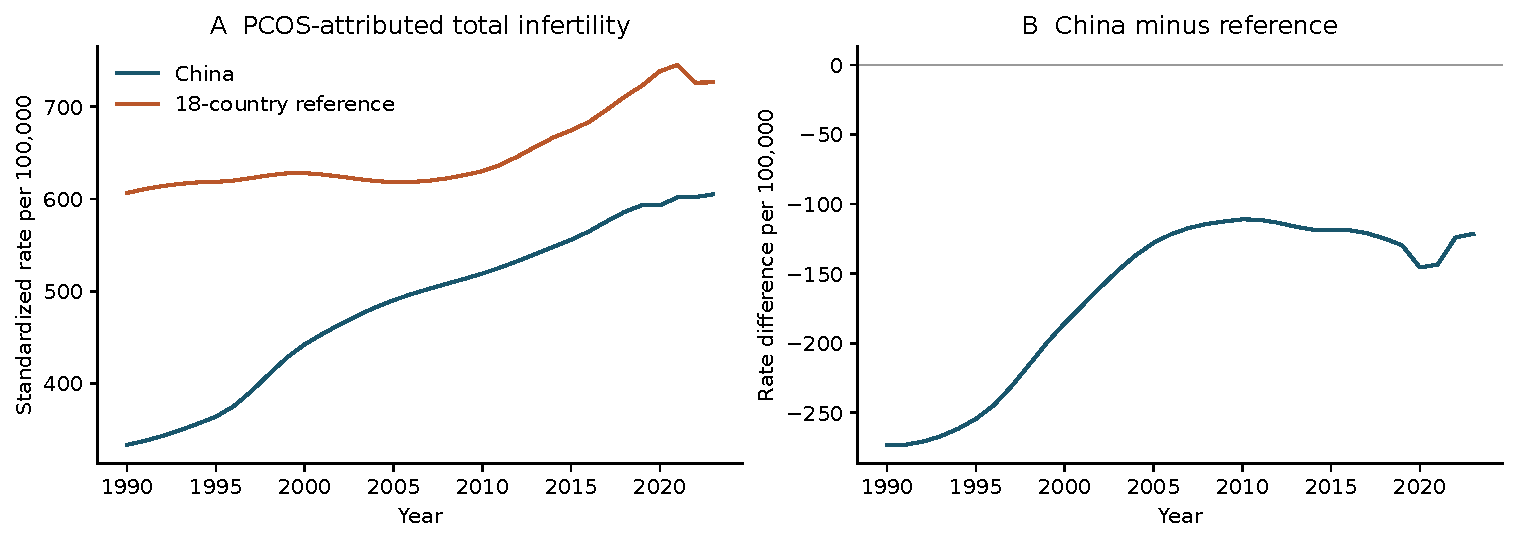
\includegraphics[width=\textwidth]{figures/Figure1_PCOS_trends.pdf}
\caption{\textbf{PCOS-attributed total infertility rates and China-minus-reference differences.} The reference pools the 18 countries within age before fixed-age standardization. Both national and reference modeled rates increase. All values are point estimates without propagated GBD uncertainty.}\label{fig:trends}
\caption*{\textbf{Alt text:} Two-panel line plot. China and the population-pooled reference both increase from 1990 to 2023; the China-minus-reference difference remains negative and narrows from minus 272.92 to minus 121.38 per 100,000.}\end{figure}
\clearpage
\begin{figure}[p]\centering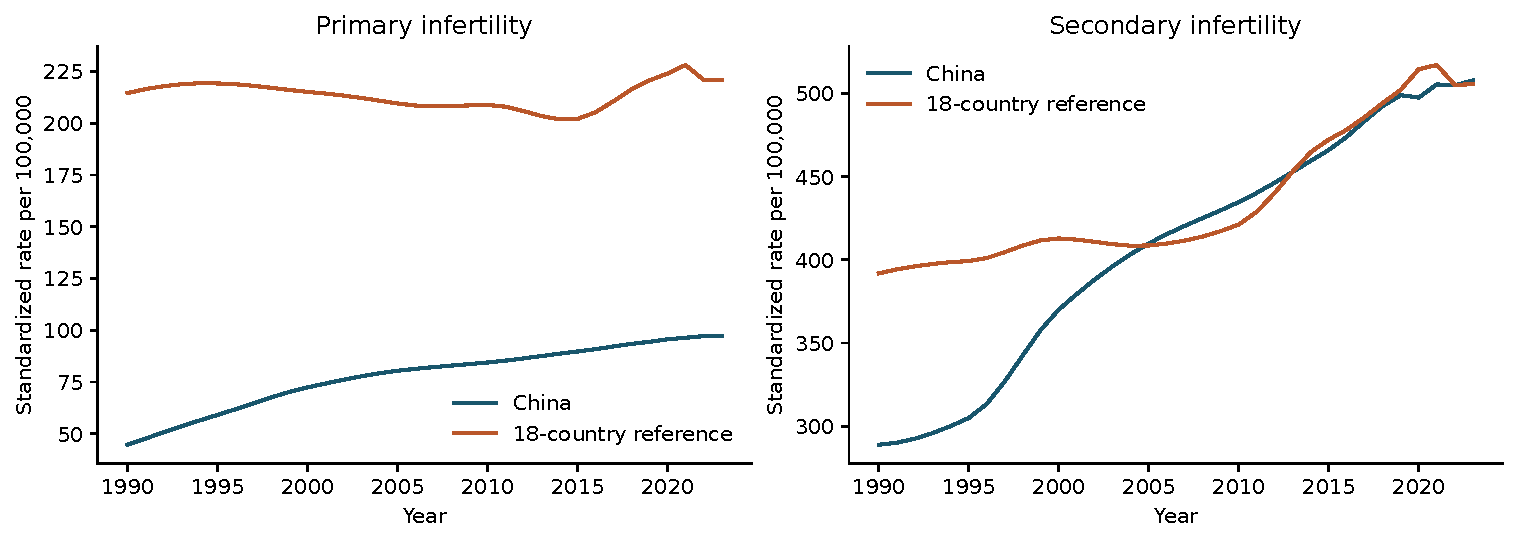
\includegraphics[width=\textwidth]{figures/Figure2_PCOS_subtypes.pdf}
\caption{\textbf{PCOS-attributed primary and secondary infertility trajectories.} The same population-pooled GBD reference and age standard are used. The categories do not track individual transitions.}\label{fig:subtypes}
\caption*{\textbf{Alt text:} Primary and secondary PCOS-attributed infertility trajectories. The primary contrast remains negative; the secondary contrast approaches zero and is plus 2.16 per 100,000 in 2023 under contemporary GBD reference shares.}\end{figure}
\clearpage
\begin{figure}[p]\centering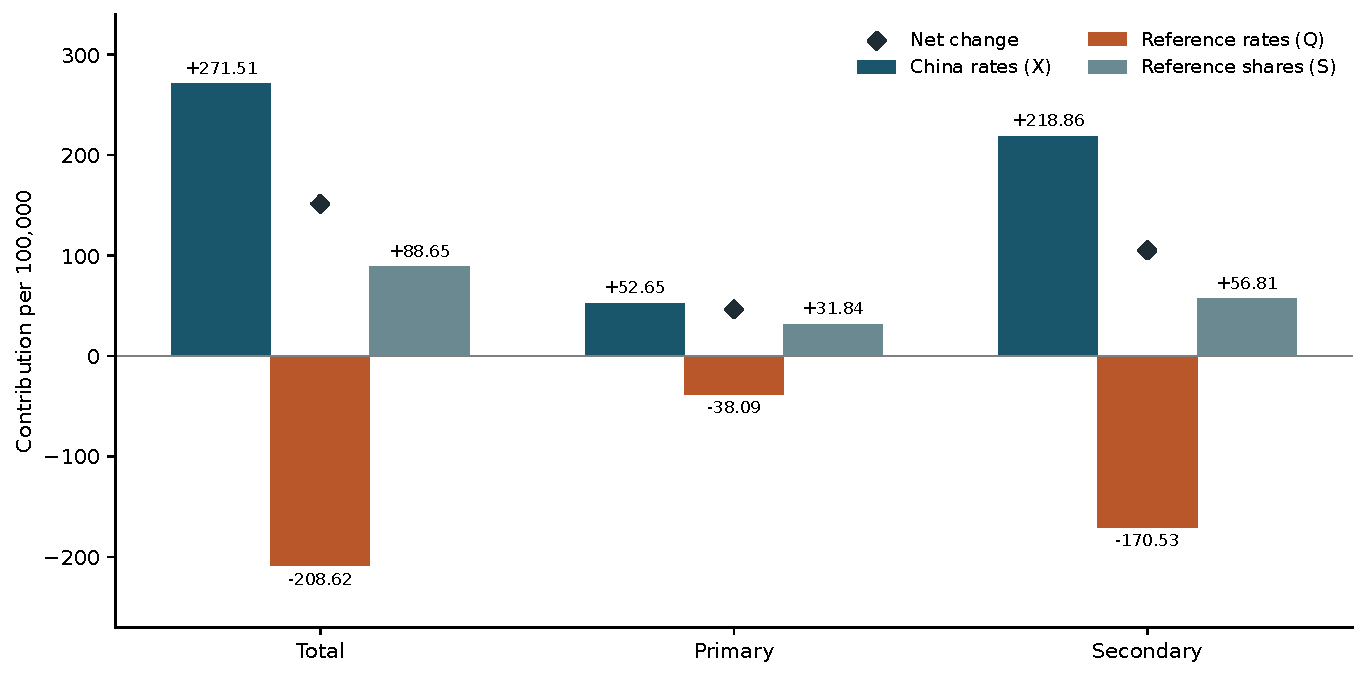
\includegraphics[width=\textwidth]{figures/Figure3_decomposition.pdf}
\caption{\textbf{Absolute symmetric components of changing PCOS contrasts, 1990--2023.} China-rate, reference-rate and reference-share components add to the diamond-marked net changes before rounding. Components with opposing signs cancel; their percentages of the net are descriptive accounting ratios.}\label{fig:decomp}
\caption*{\textbf{Alt text:} Bars separate Chinese rate, reference rate and reference share components by infertility type, with diamonds for net changes. For total infertility the components are plus 271.51, minus 208.62 and plus 88.65 per 100,000.}\end{figure}
\clearpage
\begin{figure}[p]\centering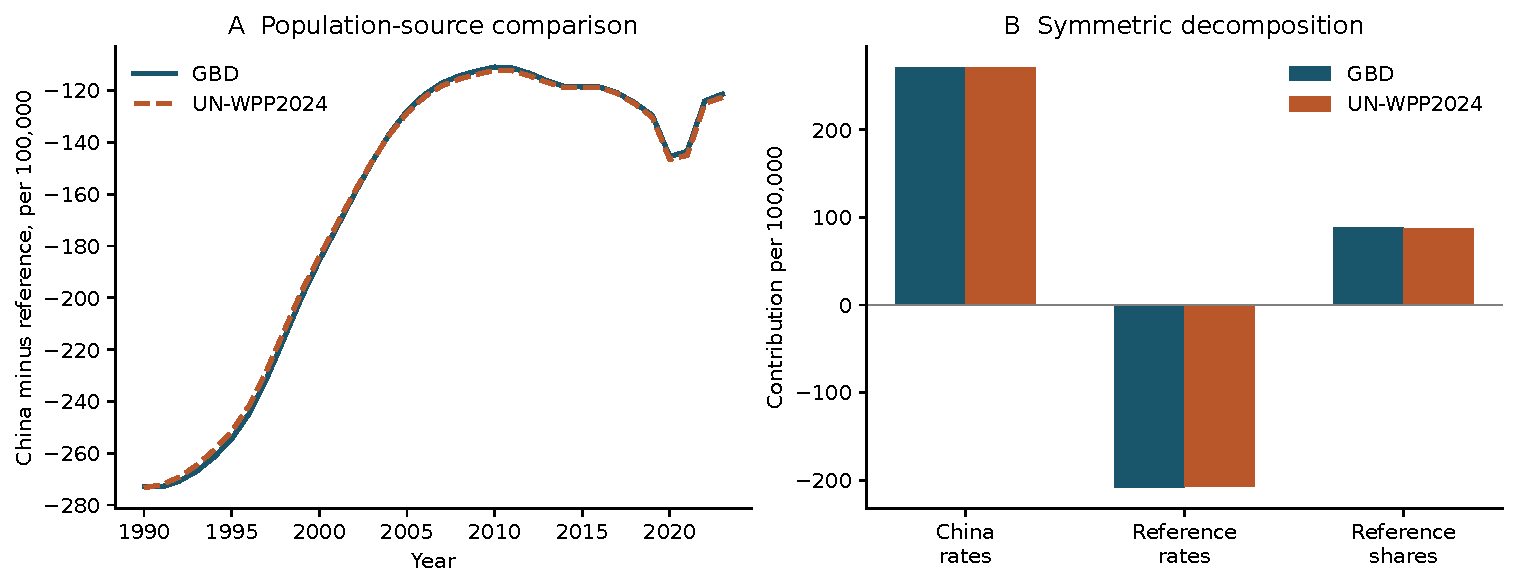
\includegraphics[width=\textwidth]{figures/Figure4_population_source.pdf}
\caption{\textbf{Alternative demographic-source weighting of the PCOS comparison.} Panel A shows annual total-infertility differences; panel B shows endpoint decomposition components. Only within-age reference-country shares change between GBD and UN scenarios; disease rates and age weights remain fixed.}\label{fig:source}
\caption*{\textbf{Alt text:} Annual differences and endpoint components under GBD and UN shares are close. For total infertility, the share component is plus 88.65 with GBD and plus 86.76 with UN; disease rates are held fixed.}\end{figure}
\clearpage
\begin{figure}[p]\centering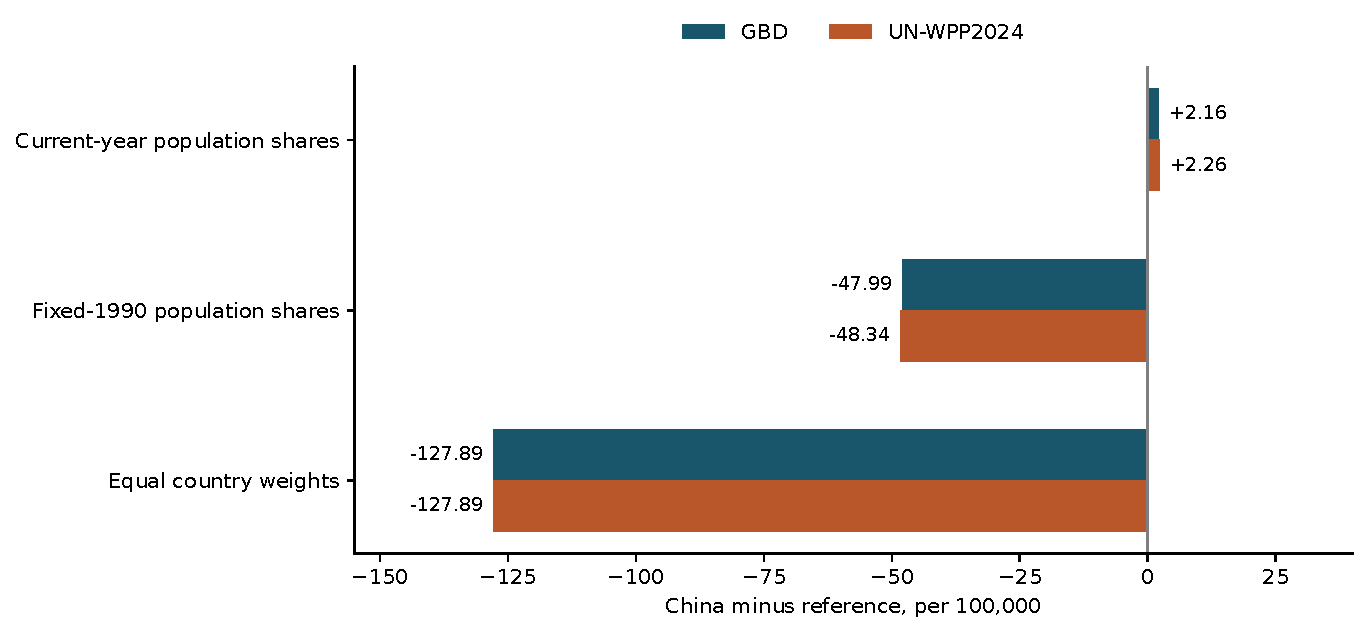
\includegraphics[width=\textwidth]{figures/Figure5_benchmark_sensitivity.pdf}
\caption{\textbf{Benchmark dependence of the 2023 PCOS secondary-infertility difference.} Current-year, fixed-1990 and equal-country reference weights answer different comparison questions. Bars show point estimates under GBD or UN population shares. Equal-country values coincide by construction; no bar represents a confidence interval.}\label{fig:bench}
\caption*{\textbf{Alt text:} Benchmark bars for secondary infertility in 2023. The GBD difference is plus 2.16 with current shares, minus 47.99 with 1990 shares and minus 127.89 with equal-country weights; UN scenarios show the same sign pattern.}\end{figure}
\clearpage

\end{document}
